%\documentclass[notheorems]{beamer}
%\documentclass[handout]{beamer}
%\documentclass[handout,notes=show]{beamer}

\usetheme{metropolis}
%\usecolortheme{dolphin}
% No navigation bars
\beamertemplatenavigationsymbolsempty
\setbeamertemplate{footline}{}


\usepackage{amsmath, amssymb, amsfonts, tikz}
\usepackage[utf8]{inputenc}
\usepackage[T1]{fontenc}
\usepackage[english]{babel}
\usepackage{tabularx}
\usepackage{mathtools}
\usepackage{xmpmulti}
\usepackage{wrapfig}
\usepackage{listings}

\makeatletter
\let\@@magyar@captionfix\relax
\makeatother
\usepackage{floatrow}
\usepackage{caption}

\definecolor{identifiers}{rgb}{0.375,0,0.375}
\definecolor{comments}{rgb}{0.5,0,0}
\definecolor{strings}{rgb}{0,0.5,0}
\definecolor{keywords}{rgb}{0,0,0.5}
%% We define a null language, free of any formatting or style
%% for use when a language is not supported, or pseudo-code
\lstdefinelanguage{none}{identifierstyle=,commentstyle=,stringstyle=,keywordstyle=}
%% A style, both text behavior and decorations all at once
\lstdefinestyle{programstyle}{breaklines=true,breakatwhitespace=true,columns=fixed,frame=leftline,framesep=3ex, xleftmargin=3ex,
basicstyle=\small\ttfamily,identifierstyle=\color{identifiers},commentstyle=\color{comments},stringstyle=\color{strings},keywordstyle=\color{keywords}}
%% The environments manufactured by the listings package
%% Two environments, one full-width, the other boxed for side-by-sides
%% "program" expects a language argument only
%% "programbox" expects a language and a linewidth
\newenvironment{listing}{\par\bigskip\noindent}{}
\lstnewenvironment{program}[1][]
  {\lstset{style=programstyle,#1}}
  {}
\lstnewenvironment{programbox}[1][]
  {\lstset{style=programstyle,#1}}
  {}


\lstdefinelanguage{Sage}[]{Python}
{morekeywords={True,False,sage,singular},
sensitive=true}
\lstset{frame=none,
          showtabs=False,
          showspaces=False,
          showstringspaces=False,
          commentstyle={\ttfamily\color{dredcolor}},
          keywordstyle={\ttfamily\color{dbluecolor}\bfseries},
          stringstyle ={\ttfamily\color{dgraycolor}\bfseries},
          language = Sage,
      basicstyle={\small \ttfamily},
      aboveskip=.3em,
      belowskip=.1em
          }
\definecolor{dblackcolor}{rgb}{0.0,0.0,0.0}
\definecolor{dbluecolor}{rgb}{.01,.02,0.7}
\definecolor{dredcolor}{rgb}{0.8,0,0}
\definecolor{dgraycolor}{rgb}{0.30,0.3,0.30}
\newcommand{\dblue}{\color{dbluecolor}\bf}
\newcommand{\dred}{\color{dredcolor}\bf}
\newcommand{\dblack}{\color{dblackcolor}\bf}

\renewcommand{\emph}[1]{{\dblack{#1}}}

\newcommand{\Sage}{{\color{dbluecolor}\sf Sage}\xspace}




\setsansfont[
    Extension      = .otf,
    UprightFont    = *-Light,
    ItalicFont     = *-LightItalic,
    BoldFont       = *-Regular,
    BoldItalicFont = *-RegularItalic
]{FiraSans}
\setmonofont[
    Extension   = .otf,
    UprightFont = *-Regular,
    BoldFont    = *-Medium
]{FiraMono}

\definecolor{Purple}{HTML}{911146}
\definecolor{Orange}{HTML}{CF4A30}
\definecolor{Tan}{RGB}{225,221,191}
\definecolor{Green}{RGB}{76,131,122}
\definecolor{DB}{RGB}{4,37,58}

% Theme colors are derived from these two elements
\setbeamercolor{alerted text}{fg=Green}

% ... however you can of course override styles of all elements
\setbeamercolor{frametitle}{bg=Tan,fg=DB}

\metroset{titleformat=smallcaps}


\newcommand{\downleadsto}{\rotatebox[origin=c]{-90}{$\leadsto$}}
\usepackage{amsthm}
\theoremstyle{plain}
\newtheorem{theorem}{Theorem}[section]
\newtheorem{corollary}[theorem]{Corollary}
\newtheorem{lemma}[theorem]{Lemma}
\newtheorem{algorithm}[theorem]{Algorithm}
\newtheorem{proposition}[theorem]{Proposition}
\newtheorem{claim}[theorem]{Claim}
\newtheorem{fact}[theorem]{Fact}
\newtheorem{conjecture}[theorem]{Conjecture}
%% Definition-like environments, normal text
%% Numbering is in sync with theorems, etc
\theoremstyle{definition}
\newtheorem{definition}[theorem]{Definition}
%% Remark-like environments, normal text
%% Numbering is in sync with theorems, etc
\theoremstyle{definition}
\newtheorem{remark}[theorem]{Remark}
\newtheorem{observation}[theorem]{Observation}
%% Example-like environments, normal text
%% Numbering is in sync with theorems, etc
\theoremstyle{definition}
\newtheorem{example}[theorem]{Example}
\newtheorem{question}[theorem]{Question}
\newcommand{\terminology}[1]{\textbf{#1}}

\newcommand{\NN}{\mathbf{N}}
\newcommand{\ZZ}{\mathbf{Z}}
\newcommand{\QQ}{\mathbf Q}
\newcommand{\CC}{\mathbf C}
\newcommand{\RR}{\mathbf R}
\newcommand{\FF}{\mathbf F}
\newcommand{\lt}{<}
\newcommand{\gt}{>}
\newcommand{\amp}{&}
\newcommand{\diff}{\mathop{}\!\mathrm{d}}
\newcommand{\ints}{\mathcal{O}}
\newcommand{\ideal}[1]{\mathfrak{#1}}
\usepackage{mathrsfs}\usepackage{cancel}
\newcommand{\Gal}[2]{\operatorname{Gal}(#1/#2)}
\newcommand{\absgal}[1]{\operatorname{Gal}(\overline{#1}/#1)}
\DeclareMathOperator{\USp}{USp}
\DeclareMathOperator{\Spec}{Spec}

\DeclareMathOperator{\rank}{rank}
\newcommand{\sheaf}[1]{\operatorname{\mathcal{#1}}}
\DeclareMathOperator{\Jac}{Jac}
\newcommand{\inv}{^{-1}}
\DeclareMathOperator{\norm}{Nm}
\DeclareMathOperator{\ord}{ord}
\DeclareMathOperator{\divisor}{div}
\DeclareMathOperator{\PP}{\mathbf{P}}
\DeclareMathOperator{\Hom}{Hom}
\DeclareMathOperator{\Mat}{Mat}
\DeclareMathOperator{\End}{End}

\newcommand{\lb}{[}
\newcommand{\rb}{]}

\setbeamerfont*{subtitle}{size=\small,shape=\scshape}

\author{Alex J. Best}
\institute{Boston University}
\date{2/7/2019}
\title{Explicit computation with Coleman integrals}
\subtitle{Journées Arithmétiques XXXI -- Istanbul University}

\begin{document}

\begin{frame}
  \titlepage

  \note[item]{Thank the audience for being awake.}
\end{frame}

%\begin{frame}
%\frametitle{Table of Contents}
%\tableofcontents[currentsection]
%\end{frame}

\begin{frame}{Coleman integration}
    \note{As number theorists it is natural to ask,}
    \begin{question}
        Is there $p$-adic analogue of (path) integration?
\end{question}
    \visible<2->{

        Given a $p$-adic space, ($\approx$ the $p$-adic solutions to some equations).
    We can locally write down power series defining a 1-form and try to integrate.}


\begin{wrapfigure}{r}{0.45\textwidth}
\visible<5->
{
    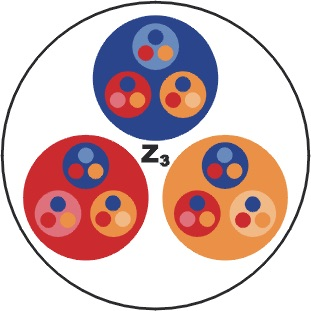
\includegraphics[width=0.45\textwidth]{padic.jpg}
}
\caption*{\visible<5->{Bad topology!}}
\end{wrapfigure}

\visible<3->{
    For instance near a point $\alpha \in \mathbf G_m(\QQ_p) = \QQ_p^\times$:
\[\frac{\mathrm d x}{x} =\frac{\mathrm{d}(\alpha+t)}{\alpha+t}=\frac{\mathrm{d} t}{\alpha+t}=\frac{1}{\alpha} \sum\left(\frac{-t}{\alpha}\right)^{n} \mathrm{d} t\]}


\visible<4->{
    so that
\[\int^{\alpha + t}_\alpha \frac{\diff x}{x} = -\sum \frac{1}{n+1}\left(\frac{-t}{\alpha}\right)^{n+1}+C\qquad\qquad\]}

\visible<5->
{
    But we cannot find $C$! There is a different choice in each disk.
}

\end{frame}

\begin{frame}{Coleman integration: More problems}
    Working on one  $p$-adic disk, the space of functions we might want to consider is
    \[T = \QQ_p\left\langle t\right\rangle=\left\{\sum a_{\mathrm{i}} t^{\mathrm{i}} ; a_{\mathrm{i}} \in \QQ_p, \lim _{\mathrm{i} \rightarrow \infty}\left|a_{\mathrm{i}}\right|=0\right\}\]
    and we have the usual differential
    \[\diff \colon T \to \Omega ^1_{T}\]
    so our integral map should send
    \[ \sum a_{i} t^{i} \diff t\mapsto\sum \frac{a_{i}}{i+1} t^{i+1} \]\pause
    but \(\frac{a_i}{i+1}\) may not converge to 0.  \pause

    $\leadsto$ Instead work with a subring, of \emph{overconvergent} functions
    \[\mathcal{T}^{\dagger}=\left\{\sum a_{\mathrm{i}} t^{\mathrm{i}} ; a_{\mathrm{i}} \in \QQ_p, \exists r>1 \text { such that } \lim _{\mathrm{i} \rightarrow \infty}\left|a_{\mathrm{i}}\right| r^{\mathrm{i}}=0\right\}\text.\]

\end{frame}


\begin{frame}{Coleman's theorem}
    Take \(X/\ZZ_p\) regular and proper, and \(p\) an odd prime.

    We pick a lift of the Frobenius map, i.e. \(\phi\colon X \to X\) which reduces to the Frobenius on $X\times_{\ZZ_p} \FF_p$, and write \(A^\dagger\) (resp.\ \(A_{\text{loc}}(X)\)) for overconvergent (resp.\ locally analytic) functions on \(X\).
    \pause%
    \begin{theorem}[{Coleman}]\label{thm-coleman-harvey-int}
        There is a \(\QQ_p\)-linear map \(\int_b^x\colon (\Omega_{A^\dagger}^1\otimes \QQ_p)^{\diff = 0} \to A_\mathrm{loc} (X)\) for which:\leavevmode%
        \[\diff \circ \int_b^x = \mathrm{id}\colon \Omega_{A^\dagger}^1\otimes \QQ_p \to \Omega_{\text{loc}}^1\,\quad\text{``FTC''}\]%
        \[\int_b^x\circ\diff = \mathrm{id}\colon A^\dagger \hookrightarrow A_{\mathrm{loc}}\]%
        \[\int_b^x \phi^*\omega = \phi^*\int_b^x \omega\,\quad\text{``Frobenius equivariance''}\]%
    \end{theorem}

    This also works over extensions of $\QQ_p$.

\end{frame}

\begin{frame}{Computation: group structure}
    If $X/\ZZ_p$ is an algebraic group, $\omega $ is a translation invariant 1-form we have

    \[\int_0^{P+Q} \omega  = \int_0^P \omega + \int_0^Q \omega \implies \int_0^{P} \omega  = \frac 1n\int_0^{nP} \omega \]

    but if $n = \# \tilde X(\FF_p)$ then $nP \in B(0,1)$ so the integral on the right can be performed locally with only power series.

    \pause
    This requires arithmetic in the group, which may be hard.
    And can only integrate invariant differentials.


\end{frame}

\begin{frame}{Computation: $p$-adic cohomology}
    There is an alternate approach via $p$-adic cohomology, due to Balakrishnan-Bradshaw-Kedlaya (for hyperelliptic curves).

    Let $X/\ZZ_p$ be a smooth curve of good reduction.

    Pick a basis $\omega_1, \ldots, \omega_{2g}$ for $H^1_\mathrm{dR}(X) = \Omega _{A^\dagger}^1/\diff(A^\dagger)$ and let $U \subseteq X$ be an affine subspace containing no poles of any $\omega_i$ and on which we have a lift of Frobenius $\phi$.\pause

    If we apply $\phi^*$ to $\omega_i$ we may write
    \[\phi^* \omega_i = \sum_{j=1}^{2g} M_{ij} \omega_j  - \diff f_i\quad\text{ using Kedlaya's algorithm, or a variant}\]\pause
    \[\implies \int_{\phi(b)}^{\phi(P)} \omega_i = \int_b^P \phi^* \omega_i = \int_b^P \left(\sum_{j=1}^{2g} M_{ij} \omega_j\right)  - \int_b^P \diff f_i\]

\end{frame}

\begin{frame}{Computation: $p$-adic cohomology}
    \[\int_{\phi(b)}^{\phi(P)} \omega_i = \int_b^P \left(\sum_{j=1}^{2g} M_{ij} \omega_j\right)  - \left( f_i(P) - f_i(b) \right)\]

    \begin{equation*}
        \implies \qquad
        \left(\begin{smallmatrix} \vdots \\ \int_{b}^{P} \omega_i \\\vdots \end{smallmatrix}\right) = (M - I)^{-1} \left(\begin{smallmatrix}\vdots \\ f_i(P) - f_i(b) \\ \vdots \end{smallmatrix}\right) \text{ if }b = \phi(b),\,P = \phi(P)
    \end{equation*}\pause
    Every point $P\in U$ is close to one fixed by Frobenius, so we can use this system and formally integrate between nearby points to find integrals with endpoints in $U$.\pause

    To move outside of $U$ we have to either work close to the boundary of the removed disks (i.e. in a highly ramified extension). Or use tricks due to the special geometry of the curve (extra automorphisms).
\end{frame}

\begin{frame}{Motivating question}
    Can $p$-adic algorithms for computing zeta functions be turned into algorithms for computing Coleman integrals? \pause

    For instance Harvey and Minzlaff have introduced variants of Kedlaya's algorithm for hyper- and super-elliptic curves that work well when $p$ is large!\pause

    They use interpolation to reduce the computation when reducing
    \[\phi^* \omega_j \leadsto \sum M_{ij} \omega_j\]
    but its not clear where the functions $f_i$ went in their work, they can simplify by forgetting this data which is irrelevant for computing zeta functions, \pause but not for Coleman integrals!

    We need to know the $f_i$ also, or, crucially, just their evaluations at points $P, b$.
\end{frame}

\begin{frame}{The reduction procedure for Superelliptic curves}
    Let \vspace{-15pt} $$ C/\ZZ_{p}\colon y^a = h(x),\,U  = C\smallsetminus \{y = 0, \infty \}$$
    with $ \gcd(a,\deg(h)) = 1$, $ p\nmid a$, \pause Minzlaff uses the lift of Frobenius $\phi $ where
    \[ \phi  (x)  = x^p,\, \phi (y)= y^p\sum_{k=0}^\infty \binom{\frac 1a}{k}\frac{(\phi(h)  - h^p)^k}{y^{apk}}\]\pause
    \[\leadsto  \phi ^* (x^i \diff x /y^j) \equiv  \sum_{k=0}^{N-1} \sum_{r=0}^{bk} \mu _{k,r,j} x^{p(i + r +1)-1} y^{-p(ak + j)} \diff x \pmod{p^N}\text.\]  \pause
    To find a cohomologous sum of basis differentials we use relations like
    \begin{align*}
        x^{i} y^{-at - \beta}\diff x -\frac{-a}{at + \beta  - a} \diff(S_i(x)y^{-at -\beta + a}) \\
        = \frac{(at + \beta - a)R_i(x) + aS'_i(x)}{at + \beta - a} y^{-a(t-1) - \beta} \diff x
    \end{align*}
    repeatedly to reduce the $y$-degree until we reach the basis.
\end{frame}


\begin{frame}
    Note that the term 
    \[
        \frac{(at + \beta - a)R_i(x) + aS'_i(x)}{at + \beta - a}
    \]
    is linear in the exponent $t$ of $y$, this is key to applying the algorithm of Bostan-Gaudry-Schost to speed up evaluation. \pause
    But the term that we must add to evaluate the $f_i$
    \[\frac{-a}{at + \beta  - a}S_i(x)y^{-at -\beta + a} \]
    is not linear in $t$! \pause
    However if we think of evaluating $f$ as follows
    \[\left(\sum_{i = 0}^N a_i y^i\right)= ((\cdots ((a_N)y + a_{N-1})y  + \cdots)y + a_0)\]
    we obtain a linear recurrence whose coefficients are fractions of linear functions of $t$.


\end{frame}


\begin{frame}{Superelliptic curves}
    \begin{theorem}[B.]
        For $X$ superelliptic as above.
        Let $ M$ be the matrix of Frobenius acting on  $ H^1_\mathrm{dR}(C)$, basis $ {\{\omega_{i,j}= x^i\diff x /y^j\}}_{i=0,\ldots, b-2,j=1,\ldots,a}$ and points $ P,Q\in C(\QQ_{p^n})$ (known to precision $ p^N$).

        If $ p \gt (aN - 1)b$, the vector of Coleman integrals $\left(\int_P^Q \omega_{i,j}\right)_{i,j}$ can be computed in time 
        $$ \widetilde O\left(g^3 \sqrt{p}n N^{5/2} + N^4 g^4 n^2 \log p \right)$$
        to absolute precision  $ N - v_p(\det(M-I))$.
    \end{theorem}
\end{frame}


\begin{frame}{Applications: Chabauty's method}
    Given $X/\QQ$ a smooth curve and $p> 2\cdot\operatorname{genus}(X)$ a prime of good reduction for $X$ and base point $b \in X(\QQ)$.
    If
    \[ \rank(\Jac(X))(\QQ) < \operatorname{genus}(X) \]
    we can find a differential $\omega _{\text{ann}}\in H^0(X, \Omega ^1)$ such that
    \[
        X(\QQ) \subseteq F^{-1}(0) \text{ for } F(z) = \int_b^z \omega_{\text{ann}}
    \]\pause
    this $F$ and its zero set can be computed explicitly in practice, giving an explicit finite set containing $X(\QQ)$ in many examples.\pause

    \emph{Note:} We can use either the group theory or $p$-adic cohomology method here.

\end{frame}

\begin{frame}{Applications: Chabauty-Kim}
    \note{many authors have tried to make this explicit and useful in examples culminating in}
    Minhyong Kim has vastly generalised the above to cases where
    \[ \rank(\Jac(X))(\QQ) \ge \operatorname{genus}(X)\]\pause
    This can be made effective, and computable
    \begin{theorem}[Balakrishnan-Dogra-Muller-Tuitman-Vonk]
        The (cursed) modular curve \(X_{split}(13)\) (of genus 3 and jacobian rank 3),
        has 7 rational points: one cusp and 6 points that correspond to CM elliptic curves whose mod-13 Galois representations land in normalizers of split Cartan subgroups.
    \end{theorem}\pause

    Their method can also be applied to other interesting curves:

    \begin{theorem}[WIP B.-Bianchi-Triantafillou-Vonk]
        The modular curve \(X_{0}(67)^+\) (of genus 2 and jacobian rank 2),
        has rational points contained in an explicitly computable set of $7$-adic points of cardinality 16.
    \end{theorem}
\end{frame}


\end{document}
